\documentclass[english]{SPFShortReport}
\usepackage{subfigure}
\usepackage{spfFigures}
\usepackage{longtable}
\usepackage{url}
\usepackage{gensymb}
\usepackage[yyyymmdd,hhmmss]{datetime}
\reportName{Python calculation for heat pump SIN-100TE}
\reportSubName{Parametric Heat Pump calculation} 
\reportDate{\today \hspace{0.1cm} at: \currenttime \hspace{0.1cm} h} 
\author{Dani Carbonell}
\address{dani.carbonell@solarenergy.ch}
\begin{document}
\begin{table}[!ht]
\begin{small}
\caption{Fitted coefficients for the heat pump.}
\begin{center}
\resizebox{12cm}{!} 
{
\begin{tabular}{l | c c } 
\hline
\hline
Coefficient &Description & \\ 
 & &$[kW]$\\ 
\hline
$PQ_{1}$ & \emph{$1^{st}$ condenser polynomial coefficient}  & 8.8992e+01    \\ 
$PQ_{2}$ & \emph{$2^{st}$ condenser polynomial coefficient}  & 6.8460e+02    \\ 
$PQ_{3}$ & \emph{$3^{st}$ condenser polynomial coefficient}  & 1.8677e+02    \\ 
$PQ_{4}$ & \emph{$4^{st}$ condenser polynomial coefficient}  & -3.6498e+02    \\ 
$PQ_{5}$ & \emph{$5^{st}$ condenser polynomial coefficient}  & 5.8326e+01    \\ 
$PQ_{6}$ & \emph{$6^{st}$ condenser polynomial coefficient}  & -9.8419e+02    \\ 
\hline
$PCOP_{1}$ & \emph{$1^{st}$ COP polynomial coefficient}  & 5.4931e+00    \\ 
$PCOP_{2}$ & \emph{$2^{st}$ COP polynomial coefficient}  & 2.4336e+01    \\ 
$PCOP_{3}$ & \emph{$3^{st}$ COP polynomial coefficient}  & 2.6236e+00    \\ 
$PCOP_{4}$ & \emph{$4^{st}$ COP polynomial coefficient}  & -1.0492e+01    \\ 
$PCOP_{5}$ & \emph{$5^{st}$ COP polynomial coefficient}  & -7.4207e+00    \\ 
$PCOP_{6}$ & \emph{$6^{st}$ COP polynomial coefficient}  & -8.8722e+01    \\ 
\hline
$\dot m_{cond}$ & 16300.00 $[kg/h]$\\ 
$\dot m_{evap}$ & 16300.00 $[kg/h]$\\ 
\hline
$COP_{nom}$ (B0W35)& 4.37 \\ 
$Q_{c,nom}$ (B0W35)& 92.43 kW\\ 
$COP_{nom}$ (B2W35)& 4.54 \\ 
$Q_{c,nom}$ (B2W35)& 96.86 kW\\ 
$COP_{nom}$ (B10W35)& 5.20 \\ 
$Q_{c,nom}$ (B10W35)& 114.61 kW\\ 
\hline
\hline
\end{tabular}
}
\label{CoefTable}
\end{center}
\end{small}
\end{table}
\begin{table}[!ht]
\begin{small}
\caption{Predicting results of the heat pump.}
\begin{center}
\resizebox{12cm}{!} 
{
\begin{tabular}{l | c c c c c c c c c c c } 
\hline
\hline
$T_{evap,in}$ &$T_{evap,out}$ &$T_{cond,in}$ &$T_{cond,out}$ &$COP$ &$Q_{cond}$ &$Q_{evap}$ &$W_{comp}$ &$\dot m_{cond}$ &$\dot m_{evap}$ &$\Delta T_{evap}$ &$\Delta T_{cond}$ \\ 
$^oC$ &$^oC$ &$^oC$ &$^oC$ &$[-]$ &$[kW]$ &$[kW]$ &$[kW]$ &kg/h &kg/h &K &K\\ 
\hline
-7.00 & -10.38 & 25.93 & 30.00 & 4.08 & 77.27 & 58.35 & 18.92 & 16300 & 16300 & 3.4 & 4.1\\ 
-7.00 & -10.16 & 34.72 & 38.75 & 3.51 & 76.40 & 54.66 & 21.74 & 16300 & 16300 & 3.2 & 4.0\\ 
-7.00 & -9.72 & 43.61 & 47.50 & 2.76 & 73.73 & 47.06 & 26.67 & 16300 & 16300 & 2.7 & 3.9\\ 
-7.00 & -8.84 & 52.59 & 56.25 & 1.84 & 69.45 & 31.77 & 37.68 & 16300 & 16300 & 1.8 & 3.7\\ 
-7.00 & -6.11 & 61.57 & 65.00 & 0.81 & 65.07 & -15.40 & 80.47 & 16300 & 16300 & -0.9 & 3.4\\ 
-4.00 & -7.74 & 25.58 & 30.00 & 4.34 & 83.92 & 64.58 & 19.34 & 16300 & 16300 & 3.7 & 4.4\\ 
-4.00 & -7.53 & 34.38 & 38.75 & 3.77 & 82.97 & 60.95 & 22.02 & 16300 & 16300 & 3.5 & 4.4\\ 
-4.00 & -7.10 & 43.27 & 47.50 & 3.02 & 80.20 & 53.62 & 26.58 & 16300 & 16300 & 3.1 & 4.2\\ 
-4.00 & -6.29 & 52.26 & 56.25 & 2.09 & 75.75 & 39.55 & 36.20 & 16300 & 16300 & 2.3 & 4.0\\ 
-4.00 & -4.13 & 61.28 & 65.00 & 1.03 & 70.66 & 2.17 & 68.49 & 16300 & 16300 & 0.1 & 3.7\\ 
-1.00 & -5.10 & 25.22 & 30.00 & 4.59 & 90.59 & 70.86 & 19.73 & 16300 & 16300 & 4.1 & 4.8\\ 
-1.00 & -4.89 & 34.03 & 38.75 & 4.02 & 89.55 & 67.27 & 22.28 & 16300 & 16300 & 3.9 & 4.7\\ 
-1.00 & -4.48 & 42.93 & 47.50 & 3.27 & 86.68 & 60.16 & 26.52 & 16300 & 16300 & 3.5 & 4.6\\ 
-1.00 & -3.72 & 51.92 & 56.25 & 2.34 & 82.10 & 47.03 & 35.07 & 16300 & 16300 & 2.7 & 4.3\\ 
-1.00 & -1.92 & 60.97 & 65.00 & 1.26 & 76.52 & 15.96 & 60.56 & 16300 & 16300 & 0.9 & 4.0\\ 
2.00 & -2.47 & 24.87 & 30.00 & 4.84 & 97.27 & 77.18 & 20.09 & 16300 & 16300 & 4.5 & 5.1\\ 
2.00 & -2.26 & 33.68 & 38.75 & 4.27 & 96.15 & 73.63 & 22.52 & 16300 & 16300 & 4.3 & 5.1\\ 
2.00 & -1.86 & 42.59 & 47.50 & 3.52 & 93.19 & 66.70 & 26.48 & 16300 & 16300 & 3.9 & 4.9\\ 
2.00 & -1.14 & 51.59 & 56.25 & 2.59 & 88.47 & 54.30 & 34.17 & 16300 & 16300 & 3.1 & 4.7\\ 
2.00 & 0.41 & 60.65 & 65.00 & 1.50 & 82.53 & 27.50 & 55.04 & 16300 & 16300 & 1.6 & 4.4\\ 
5.00 & 0.16 & 24.52 & 30.00 & 5.09 & 103.96 & 83.54 & 20.42 & 16300 & 16300 & 4.8 & 5.5\\ 
5.00 & 0.37 & 33.33 & 38.75 & 4.52 & 102.76 & 80.02 & 22.74 & 16300 & 16300 & 4.6 & 5.4\\ 
5.00 & 0.76 & 42.24 & 47.50 & 3.77 & 99.71 & 73.24 & 26.47 & 16300 & 16300 & 4.2 & 5.3\\ 
5.00 & 1.45 & 51.25 & 56.25 & 2.84 & 94.87 & 61.42 & 33.46 & 16300 & 16300 & 3.6 & 5.0\\ 
5.00 & 2.82 & 60.33 & 65.00 & 1.74 & 88.66 & 37.65 & 51.01 & 16300 & 16300 & 2.2 & 4.7\\ 
8.00 & 2.79 & 24.17 & 30.00 & 5.34 & 110.67 & 89.94 & 20.73 & 16300 & 16300 & 5.2 & 5.8\\ 
8.00 & 3.00 & 32.98 & 38.75 & 4.77 & 109.39 & 86.44 & 22.95 & 16300 & 16300 & 5.0 & 5.8\\ 
8.00 & 3.38 & 41.90 & 47.50 & 4.01 & 106.24 & 79.78 & 26.46 & 16300 & 16300 & 4.6 & 5.6\\ 
8.00 & 4.04 & 50.91 & 56.25 & 3.08 & 101.30 & 68.42 & 32.87 & 16300 & 16300 & 4.0 & 5.3\\ 
8.00 & 5.29 & 60.00 & 65.00 & 1.98 & 94.85 & 46.89 & 47.97 & 16300 & 16300 & 2.7 & 5.0\\ 
11.00 & 5.42 & 23.81 & 30.00 & 5.58 & 117.39 & 96.37 & 21.02 & 16300 & 16300 & 5.6 & 6.2\\ 
11.00 & 5.62 & 32.63 & 38.75 & 5.01 & 116.03 & 92.88 & 23.15 & 16300 & 16300 & 5.4 & 6.1\\ 
11.00 & 6.00 & 41.55 & 47.50 & 4.26 & 112.80 & 86.32 & 26.48 & 16300 & 16300 & 5.0 & 5.9\\ 
11.00 & 6.64 & 50.57 & 56.25 & 3.33 & 107.74 & 75.35 & 32.40 & 16300 & 16300 & 4.4 & 5.7\\ 
11.00 & 7.79 & 59.67 & 65.00 & 2.22 & 101.11 & 55.50 & 45.60 & 16300 & 16300 & 3.2 & 5.3\\ 
14.00 & 8.05 & 23.46 & 30.00 & 5.83 & 124.13 & 102.83 & 21.29 & 16300 & 16300 & 6.0 & 6.5\\ 
14.00 & 8.25 & 32.28 & 38.75 & 5.26 & 122.68 & 99.35 & 23.33 & 16300 & 16300 & 5.8 & 6.5\\ 
14.00 & 8.63 & 41.21 & 47.50 & 4.50 & 119.37 & 92.87 & 26.50 & 16300 & 16300 & 5.4 & 6.3\\ 
14.00 & 9.24 & 50.23 & 56.25 & 3.57 & 114.21 & 82.21 & 32.00 & 16300 & 16300 & 4.8 & 6.0\\ 
14.00 & 10.31 & 59.34 & 65.00 & 2.46 & 107.41 & 63.68 & 43.72 & 16300 & 16300 & 3.7 & 5.7\\ 
17.00 & 10.67 & 23.10 & 30.00 & 6.07 & 130.88 & 109.32 & 21.55 & 16300 & 16300 & 6.3 & 6.9\\ 
17.00 & 10.87 & 31.93 & 38.75 & 5.50 & 129.36 & 105.84 & 23.52 & 16300 & 16300 & 6.1 & 6.8\\ 
17.00 & 11.25 & 40.86 & 47.50 & 4.75 & 125.95 & 99.42 & 26.53 & 16300 & 16300 & 5.8 & 6.6\\ 
17.00 & 11.85 & 49.89 & 56.25 & 3.81 & 120.70 & 89.02 & 31.67 & 16300 & 16300 & 5.2 & 6.4\\ 
17.00 & 12.86 & 59.00 & 65.00 & 2.70 & 113.74 & 71.54 & 42.20 & 16300 & 16300 & 4.1 & 6.0\\ 
20.00 & 13.30 & 22.74 & 30.00 & 6.31 & 137.64 & 115.84 & 21.80 & 16300 & 16300 & 6.7 & 7.3\\ 
20.00 & 13.50 & 31.58 & 38.75 & 5.74 & 136.04 & 112.35 & 23.69 & 16300 & 16300 & 6.5 & 7.2\\ 
20.00 & 13.87 & 40.51 & 47.50 & 4.99 & 132.56 & 105.98 & 26.57 & 16300 & 16300 & 6.1 & 7.0\\ 
20.00 & 14.46 & 49.54 & 56.25 & 4.05 & 127.20 & 95.80 & 31.40 & 16300 & 16300 & 5.5 & 6.7\\ 
20.00 & 15.42 & 58.67 & 65.00 & 2.93 & 120.11 & 79.16 & 40.95 & 16300 & 16300 & 4.6 & 6.3\\ 
\hline
\hline
\end{tabular}
}
\label{ResultsTable}
\end{center}
\end{small}
\end{table}
\begin{figure}[!ht]
\begin{center}
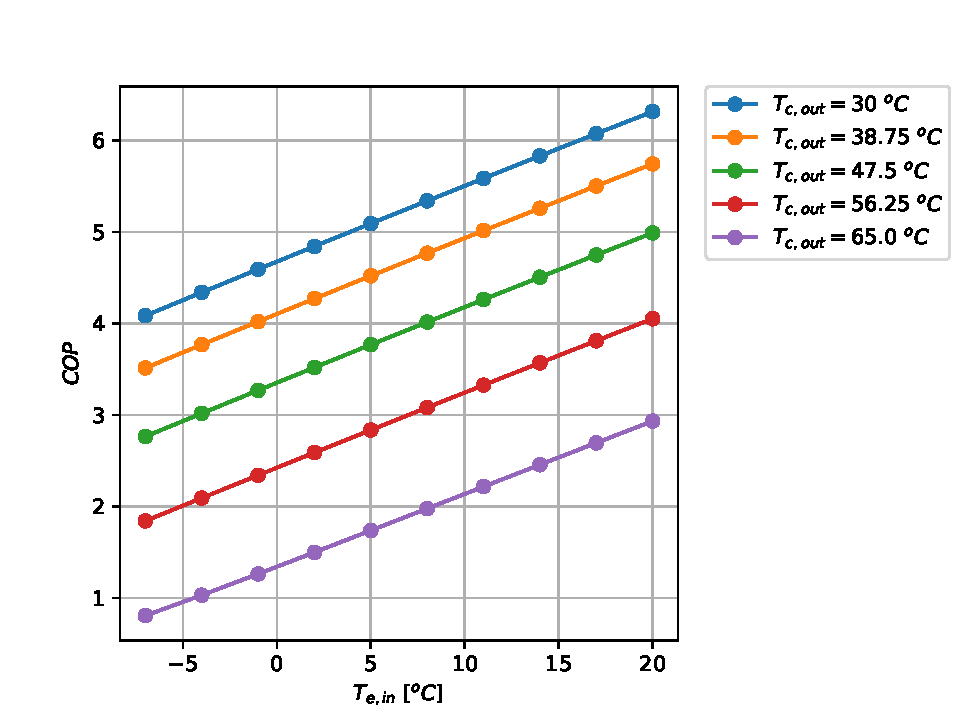
\includegraphics[width=1\textwidth]{C:/Daten/spfPackages/GIT/spfTrnsysFiles/HeatPump/BrineToWater/Walter Meier/SIN-100TE/SIN-100TE-Cop.pdf}
\caption{COP Results for the heat pump at the selected points}
\label{COPFig}
\end{center}
\end{figure}
\begin{figure}[!ht]
\begin{center}
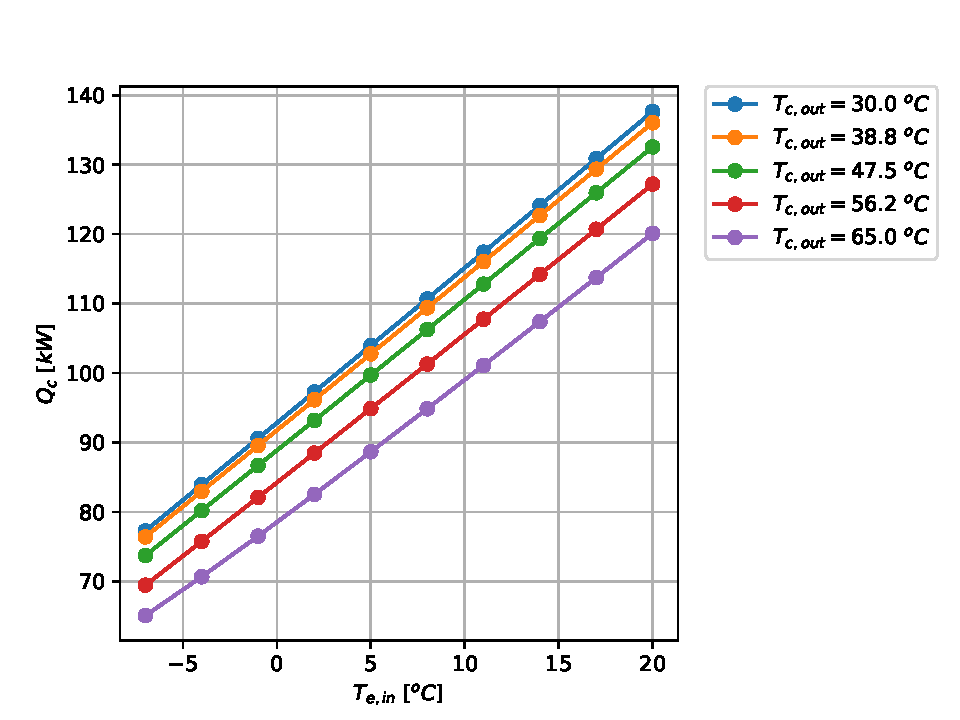
\includegraphics[width=1\textwidth]{C:/Daten/spfPackages/GIT/spfTrnsysFiles/HeatPump/BrineToWater/Walter Meier/SIN-100TE/SIN-100TE-Qc.pdf}
\caption{$Q_c$ Results for the heat pump at the selected points}
\label{QcFig}
\end{center}
\end{figure}
\end{document}
